%----------------------------------------------------------------
%
%  File    :  state_of_the_art.tex
%
%  Authors :  David Lechner, FH Campus Wien, Austria
%
%  Created :  10 Oct 2019
%
%  Changed :  10 Oct 2019
%
%----------------------------------------------------------------


\chapter{Grundlagen}
\label{chap:state_of_the_art}

In diesem Kapitel werden die Grundlagen für das zu realisierende System beschrieben. Es beinhaltet eine Einführung in \textit{Machine Learning}\footnote{Informationen aus \cite{Rebala2019}} und gibt dabei einen Überblick auf die verschiedenen Methoden und Anwendungsfälle. Speziell werden Algorithmen beschrieben, welche laut Literatur\footnote{\cite{Gahr2018}, \cite{Hallac2016}} besonders interessant für dieses Thema sind. Zudem wird der \textit{Controller Area Network} Bus vorgestellt, welcher für die Datensammlung im Kontext der Masterarbeit essenziell ist.

\section{Machine Learning}
\label{sec:machine_learning}

\textit{Machine Learning} ist ein Bereich der Computer Wissenschaften und beschäftigt sich mit Algorithmen und Techniken zur Lösung von komplexen Problemen, wo konventionelle Programmiermethoden nicht vielversprechend sind. Wir werden heutzutage im alltäglichen Leben mit vielen Anwendungen konfrontiert, die ohne ML nicht möglich wären. Beispiele dafür sind Sprachsteuerung, Bild-, Gesichts- und Handschrifterkennung, Stauvorhersage aber auch Autonomes Fahren und die Erkennung von Brustkrebs \cite{KOUROU20158}. Schon vor 1980 wurde versucht, einige solcher komplexen Probleme zu lösen, was jedoch nicht immer von Erfolg gekrönt war. Erst Mitte der 2000er Jahre ist der Fortschritt in dem Bereich drastisch gestiegen. Gründe dafür gibt es mehrere. Zum einen ist mit dem Aufkommen des Internets eine viel größere Anzahl an Daten vorhanden und zum anderen sind Rechenleistung beziehungsweise Speicherplatz billiger, leichter zugänglich und vor allem performanter. Des Weiteren sind die Algorithmen verbessert und angepasst worden.

Oft werden \textit{Machine Learning} und Künstliche Intelligenz (engl. \textit{Artificial Intelligence}, kurz AI) mit einander gleichgesetzt, was jedoch nicht stimmt. AI ist ein viel breitgefächerter Forschungsbereich, der mittels mehrerer Ansätzen versucht, Maschinen das "Denken" beizubringen. ML hingegen ist ein möglicher Ansatz dafür.

Um das Vorgehen zum Lösen eines komplexen Problems mittels \textit{Machine Learning} besser verstehen zu können, wird es im Folgenden anhand einer Anwendung, welche handgeschriebene Buchstaben erkennt, erklärt. Zu aller erst wird eine Vielzahl an verschiedenen Datenpunkten (engl. \textit{data points}) - Bilder mit handgeschriebenen Buchstaben - benötigt. Zusätzlich müssen diese mit den enthaltenen Buchstaben markiert (engl. \textit{labelled}) sein. Das Ziel ist, dass die Anwendung nicht nur die Buchstaben im Datenset erkennt, sondern auch jene, die nicht enthalten sind. Mit der konventionellen Methode wird anfangs versucht zu verstehen, wie die Bilder mit den Buchstaben zusammenhängen. Danach wird eine Reihe an Regeln festgelegt, um auch neue Bilder erkennen zu können. Da es jedoch eine große Variation von Handschriften gibt, kann das Regelset sehr schnell sehr groß werden. \textit{Machine Learning} Algorithmen gehen hierbei einen generelleren Lösungsweg, indem sie direkt von den markierten Daten lernen und sich das Regelset (engl. \textit{model}) selbst aneignen. Je mehr Bilder von Buchstaben vorhanden sind, desto genauer wird das ML-\textit{Model}. Werden neue Bilder ohne Markierung hinzugefügt, kann das \textit{Model} die Buchstaben erkennen. Diese Art um das Problem zu lösen wird im Kontext von ML als Klassifizierung bezeichnet. Es gibt auch noch zwei weitere, welche adressiert werden:
\begin{itemize}
  \item Prognose (engl. \textit{Prediction} oder \textit{Regression}): Trainieren eines \textit{Models} mit historischen Daten zur Vorhersage zukünftiger Werte. Z.B. der Bedarf eines bestimmten Produktes in den Sommerferien.
  \item Klassifizierung (engl. \textit{Classification}): Datenpunkte in eine oder mehrere Kategorien bzw. Klassen einteilen. Z.B. Identifizierung einer Email als Spam oder nicht, Erkennen welches Tier auf einem Bild zu sehen ist (Katze, Hund, Löwe, \dots).
  \item Gruppierung (engl. \textit{Clustering}): Unterteilung vieler Datenpunkte in wenige Gruppen, in denen Punkte mit gleichen Eigenschaften enthalten sind. Im Gegensatz zur Klassifizierung ist die Anzahl der Gruppen im Vorhinein nicht bekannt.
\end{itemize}

Zur besseren Vorstellung veranschaulicht Abbildung \ref{fig:ml_problem_types} die Arten. Abschnitt \ref{sec:ml_regression} und folgende gehen darauf näher ein.

\begin{figure}[htbp]
	\centering
		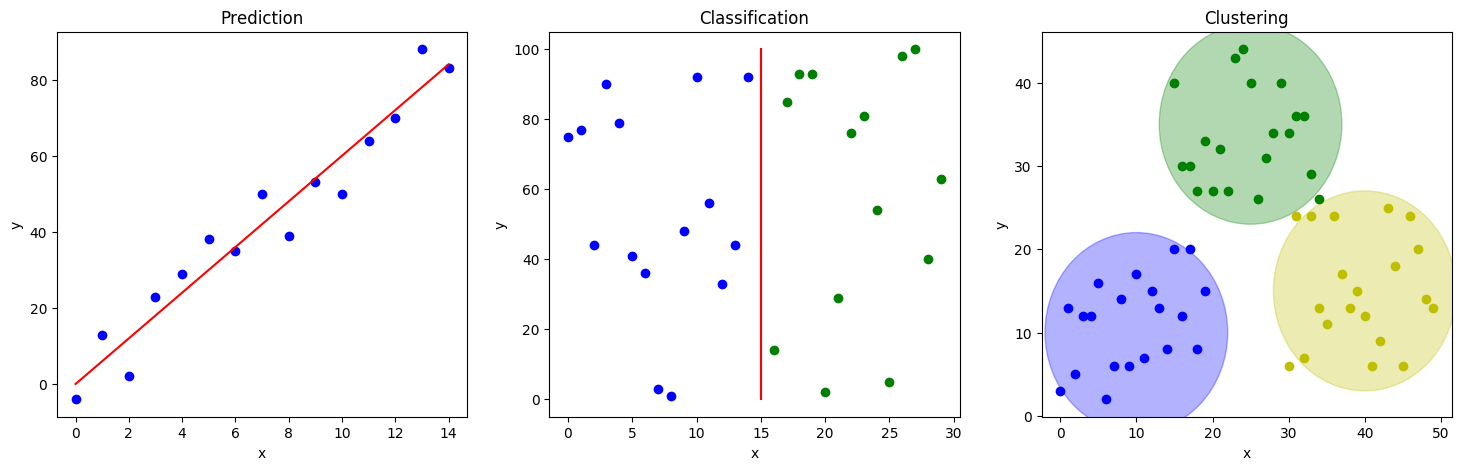
\includegraphics[width=\textwidth]{images/ml_problem_types.png}
	\caption{Arten von \textit{Machine Learning} Problemen}
	\label{fig:ml_problem_types}
\end{figure}


\subsection{Ansätze}
\label{sec:ml_types}

Um ein ML-\textit{Model} anzulernen, gibt es verschiedene Möglichkeiten. An eine davon - das Überwachte Lernen - wurde bereits in der Einführung anhand eines Beispiels herangeführt. Dieses Unterkapitel geht auch auf die anderen Möglichkeiten ein.

\subsubsection{Überwachtes Lernen}
Beim Überwachten Lernen (engl. \textit{supervised learning}) wird dem \textit{Model} ein Datenset bestehend aus Datenpunkten und den dazugehörigen korrekten Antworten zu einer Frage übergeben. Der ML-Algorithmus versucht aufgrund der Eigenschaften eines Datenpunktes einen Zusammenhang zu der Antwort zu finden. Wenn daraufhin neue Datenpunkte hinzugefügt werden, kann das \textit{Model} basierend auf den Eigenschaften eine Antwort prognostizieren. Das folgende abstrakte Beispiel demonstriert wie \textit{supervised learning} funktioniert.

Seit der Geburt lernt ein Kind, wie bestimmte Objekte aussehen und wie sie heißen. Es sieht jeden Tag einen Hund in verschiedenen Positionen, mal sitzend, laufend, stehend usw. Dadurch kann es auch den Nachbarshund als solchen identifizieren und zu einer Katze unterscheiden. Während der Lernphase kann natürlich auch ein Fehler vorkommen und das Kind kann zum Beispiel einen Wolf als einen Hund missinterpretieren. Doch die Eltern und Geschwister erklären dem Kind, dass es sich dabei nicht um einen Hund handelt. Es passt daher das Verständnis an und wird immer besser, das Tier zu identifizieren. Im Kontext von ML ist die oben beschrieben Anwendung zur Erkennung von handgeschriebenen Buchstaben genauso überwachtes Lernen.

\subsubsection{Nicht-Überwachtes Lernen}
Bei dieser Art des Lernens sind im Datenset nicht die korrekten Antworten zu den einzelnen Datenpunkten enthalten. Der Algorithmus ist darauf ausgelegt Trends zu erkennen und Datenpunkte mit Gemeinsamkeiten zu gruppieren, ohne zu wissen, worum es sich dabei handelt. Um auf das oben beschrieben Beispiel mit dem Hund zurückzukommen, werden in einem \textit{Model} viele Bilder von verschiedenen Tieren eingespielt. Die Bilder sind jedoch nicht mit dem darauf enthaltenen Tier markiert. Nachdem der Algorithmus alle Charakteristiken der Bilder analysiert hat, ist das \textit{Model} in der Lage, gleichartige Bilder zusammenzufassen. Es kann somit eine Gruppe erstellen, die alle Hunde enthält und eine andere, der alle Katzen zugeordnet sind. Am Ende hat das ML-\textit{Model} noch immer keine Vorstellung, um welches Tier es sich tatsächlich handelt.

Ein anderes Beispiel ist in der Analyse von Kaufverhalten zu finden. Das Datenset besteht hierbei aus den verschiedenen gekauften Produkten der Kunden und das Ziel ist Korrelationen darin zu finden. Das \textit{Model} soll in der Lage sein zum Beispiel folgendes bestimmen zu können: Kunden die Schultaschen kaufen, kaufen auch Stifte. Oder Kunden die Bier kaufen, kaufen auch Chips.

\subsubsection{Teil-Überwachtes Lernen}
Teil-Überwachtes Lernen (engl. \textit{semi-supervised learning}) liegt zwischen den beiden vorher beschriebenen Arten des Lernens. Es wird ein Datenset verwendet, das hauptsächlich aus unmarkierten Datenpunkten besteht. Ein kleiner Teil davon hat jedoch eine Markierung. Im ersten Schritt kommen Techniken zur Gruppierung zum Einsatz, um gleichartige Datenpunkte zu bündeln. Der zweite Schritt besteht darin, die bereits bekannten Datenpunkte dazu zu verwenden, andere Daten in der gleichen Gruppe zu markieren. Einer der größten Vorteile davon ist, dass nicht viel Zeit für das manuelle Markieren von Daten aufgewendet werden muss. Der Nachteil ist aber, dass es im Vergleich zum Überwachten Lernen komplexer ist.

Auch hier lässt sich das Beispiel mit den Tieren anwenden. Aus Zeit- oder anderen technischen Gründen können nicht alle Bilder von Hunden und Katzen durchgesehen und markiert werden. Bei ein paar ist es jedoch möglich. Beim Teil-Überwachten Lernen gruppiert zuerst das ML-\textit{Model} alle Bilder mit Hunden und Katzen (gleiche Eigenschaften). Danach können aus den paar Markierten alle anderen abgeleitet werden.

\subsubsection{Bestärkendes Lernen}
Die letzte hier vorgestellte Art ist bestärkendes Lernen (engl. \textit{reinforcement learning}). Es kommt einerseits zum Einsatz, wenn sich die Situationen fortlaufend ändern, zum Beispiel beim Autofahren oder bei einem Spiel. Das \textit{Model} muss sich hierbei immer an neue Bedingungen anpassen. Andererseits wird es auch verwendet, wenn ein großer Zustandsraum existiert. Bei beispielsweise Schach ist es kaum möglich mittels \textit{brute-force} den besten nächsten Zug herauszufinden, da es viel zu viele Möglichkeiten im Verlauf eines Spieles gibt. Der Algorithmus ist also darauf ausgelegt eine Entscheidung basierend auf dem momentanen internen Zustand und der Umgebung zu treffen, um ein vordefiniertes Ziel zu erreichen. Ein Ziel kann gegebenenfalls sein, ein Auto innerhalb der Spur zu halten. Je länger der Algorithmus lernen kann, desto besser und genauer werden die Entscheidungen in Hinblick auf eine langfristige Auswirkung.

\subsection{Regression}
\label{sec:ml_regression}

Die Regressionsanalyse (engl. \textit{regression analysis}) ist eine auf Statistik basierende \textit{Machine Learning}-Technik, welche aufgrund von oftmals historischen Daten zur Vorhersage verwendet wird. Dabei werden Relationen in markierten Daten analysiert, um eine Prognose für bestimmte Eigenschaften treffen zu können. Zum Beispiel kann damit ein \textit{Model} erstellt werden, welches den aktuellen Preis einer Immobilie bestimmt. Die historischen markierten Daten können hier die Eigenschaften Quadratmeteranzahl, Nachfrage, Lage als Kategorie, Kaufpreis, Verkaufspreis etc. haben. Im Kontext von ML werden die Eigenschaften als \textit{Features} bezeichnet. Da die Problemstellung in der Masterarbeit eine Klassifizierung erfordert, wird nur ein Algorithmus kurz vorgestellt.

\subsubsection{Linear Regression}
\label{sec:linear_regression}

Bei dieser Art der Regression wird versucht, den Wert einer kontinuierlichen Variable vorherzusagen, beispielsweise den Tagesendkurs eines bestimmen Unternehmens an der Börse. Einfachheitshalber wird angenommen, dass der aktuelle Aktienkurs nur von den Kursen und dem Volumen der letzten zehn Tage abhängt. Das ML-\textit{Model} würde daher auf der folgenden Formel basieren:

\begin{math}
	\centering
	Kurs = Konstante + a * Kurs\textsubscript{Tag-1} + b * Volumen\textsubscript{Tag-1} + c * Kurs\textsubscript{Tag-2} + d * Volumen\textsubscript{Tag-2} + \dots + s * Kurs\textsubscript{Tag-10} + t * Volumen\textsubscript{Tag-10}
	\label{formular:stock1}
\end{math}

Wenn die Koeffizienten \textit{a}, \textit{b}, \textit{c}, etc. bekannt sind, kann der Kurswert an Tag X berechnet werden. Hierfür werden historische Daten verwendet. Sie bestehen jeweils aus einem \textit{Input}/\textit{Output} Paar. Die \textit{Input} Daten sind die letzten zehn Kurswerte und Volumina und \textit{Output} ist der Kurswert am dazugehörigen Tag. Wenn der Wert der Koeffizienten ermittelt wird, der die meisten historischen Daten mit akzeptablen Fehlern erfüllt, kann das \textit{Model} den Aktienkurs des nächsten Tages vorhersagen. Da ausschließlich markierte Daten zum Lernen verwendet werden, fällt lineare Regression unter überwachtes Lernen.

\subsection{Classification}
\label{sec:classification}

Wie bereits in der Einleitung des Kapitels beschrieben, geht es bei der Klassifizierung um das Einteilen von Datenpunkten in vordefinierte Kategorien. Es fällt ebenfalls unter \textit{supervised learning}, da die Modelle mit bereits kategorisierten Daten trainiert werden. Ein \textit{Classifier} kann entweder binäre Entscheidungen treffen oder aus einem Set von Kategorien wählen.

\subsubsection{Logistic Regression}
\label{sec:logistic_regression}

\textit{Logistic Regression} kommt zum Einsatz, wenn der Prognoseraum binär ist - also 0 oder 1, ja oder nein. Um auf das vorherige Beispiel mit den Aktienkursen zurückzukommen: Eine Anwendung soll herausfinden, ob der morgige Aktienwert höher ist, als der heutige. Es könnte durchaus mit der linearen Regression ebenso erreicht werden, indem man den aktuellen Wert mit dem prognostizierten vergleicht. Jedoch ist logische Regression für solche Problemstellungen die bessere Methode.

\subsubsection{Random Forest}
\label{sec:random_forest}

Der Algorithmus \textit{Random Forest} gilt als einer der effektivsten und intuitivsten, wenn es um das Lösen von Klassifizierungsproblemen geht. Er basiert auf sogenannten \textit{Decision Trees}, welche anhand der \textit{Features} einen Entscheidungsbaum aufbauen. Mehrere von diesen bilden einen \textit{Forest}. Ein \textit{Decision Tree} ist eine Baumstruktur bestehend aus Knoten (engl. \textit{Node}), welche eine deterministische Entscheidung basierend auf Variablen treffen, und Kanten, welche zum nächsten Knoten oder zum sogenannten \textit{leaf node} führen. Dieser letzte Knoten stellt das Ergebnis dar, beziehungsweise die resultierende Klasse.

Zum Beispiel besteht ein Datenset aus Bildern von Fortbewegungsmitteln. Mithilfe einiger Fragen, welche sich auf die \textit{Features} beziehen, über ein Objekt soll herausgefunden werden, ob es sich dabei um ein Auto oder ein Fahrrad handelt. Diese Fragen könnten sein: Hat es einen Motor(?), können mehr als eine Person es benutzen(?), hat es ein Lenkrad(?), wie viele Reifen hat es(?). Jeder Knoten repräsentiert eine dieser Fragen und dessen Kanten führen zum nächsten basierend auf der Antwort. Wenn alle Fragen richtig beantwortet sind, führt der letzte Knoten zum Ergebnis - also ob auf dem Bild ein Auto oder ein Fahrrad zu sehen ist. Abbildung \ref{fig:decision_tree} zeigt einen \textit{Decision Tree} in einer vereinfachten Form.

\begin{figure}[htbp]
	\centering
		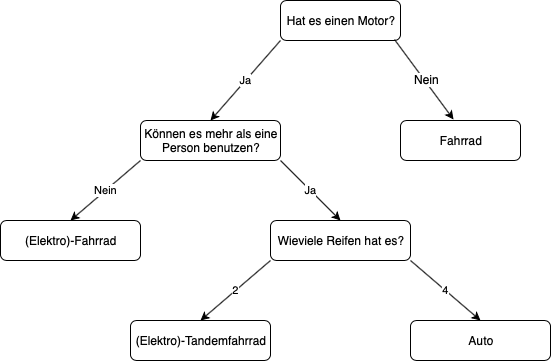
\includegraphics[width=0.8\textwidth]{images/decision_tree.png}
	\caption{Beispiel \textit{Decision Tree}}
	\label{fig:decision_tree}
\end{figure}

Das Ziel eines \textit{Decision Trees} ist also ein ML-\textit{Model} mit Entscheidungsregeln basierend auf Trainingsdaten zu erstellen. Anhand dieser Regeln soll eine Kategorie vorhergesagt werden können. Die Erstellung erfolgt dabei in drei Schritten:

\begin{description}
	\item[Schritt 1] Verwende das Attribut oder \textit{Feature} mit der größten Bedeutung als \textit{root}.
	\item[Schritt 2] Erstelle eine Entscheidung mit dem höchsten Informationsgehalt.
	\item[Schritt 3] Wiederhole rekursiv Schritt 1 und 2 bis der Baum fertig aufgebaut ist und es keine Informationen mehr zum Aufteilen gibt.
\end{description}

Wenn viele \textit{Features} in einem Datenset vorhanden sind, ist die größte Herausforderung, die beste Variable oder eine Kombination aus mehreren für einen Knoten zu finden (für Schritt 2). Dieser Vorgang wird \textit{attribute selection} genannt und wird entweder durch \textit{information gain} oder \textit{Gini Impurity} durchgeführt. Ersteres kommt eher zum Einsatz, wenn die \textit{Output}-Variable eine Kategorie ist (z.B.: Fortbewegungsmittel) und zweiteres wenn sie numerisch und kontinuierlich ist (z.B.: Alter einer Person).

In der Informationstheorie kann der Informationsgehalt einer Variable mithilfe der Entropie bestimmt werden. Wenn die Auftrittswahrscheinlichkeit eines Wertes klein ist, ist der Informationsgehalt hoch. Bei einer großen Wahrscheinlichkeit sinkt der Informationsgehalt. Entropie ist nun die Summe aller Auftrittswahrscheinlichkeiten der möglichen Werte und wird mit der Formel \ref{formular:entropy} berechnet. So hat zum Beispiel ein Würfelwurf eine höhere Entropie (2,58) als ein Münzwurf (1) und würde den Vorzug bei dem Aufteilen eines Datensets erhalten.

\begin{equation}
	H = -\sum \limits_{i=1}^n (p_i log_2 p_i)
	\label{formular:entropy}
\end{equation}

\noindent
wobei

\noindent
$p_i$ ist die Auftrittswahrscheinlichkeit des \textit{i}ten-Elements.

\noindent
$n$ ist die Anzahl an möglichen Werten.

\noindent
$H$ ist die Entropie.

Das \textit{Gini Impurity Criterion} auf der anderen Seite bestimmt die Wahrscheinlichkeit wie oft ein zufällig gewählter Datenpunkt aufgrund eines bestimmen \textit{Features} falsch klassifiziert wird. Je kleiner dieser Wert ausfällt, desto besser eignet sich das \textit{Feature} zum Aufteilen bei einem Knoten und wird bevorzugt. Die vereinfachte Formel hierfür ist:

\begin{equation}
	Ic(p) = 1 - \sum \limits_{i=1}^J p_i^2
	\label{formular:gini}
\end{equation}

\noindent
wobei

\noindent
$Ic(p)$ ist die \textit{Gini Impurity}.

\noindent
$p_i$ ist die Wahrscheinlichkeit des \textit{i}ten-Elements.

\noindent
$J$ ist Anzahl der Kategorien.

Ein \textit{Random Forest} bestimmt nun durch ein Mehrheitsvotum der Ergebnisse aus den verschiedenen \textit{Decision Trees} die höchstwahrscheinlich zutreffende Kategorie. Abbildung \ref{fig:random_forest} veranschaulicht dies. Würde jeder \textit{Tree} mit den gleichen Daten und Parametern trainiert werden, ist das Ergebnis überall das gleiche und es ergibt sich dadurch kein Vorteil. Es kommt daher \textit{Data Bagging} zum Einsatz. Dabei wird für jeden Baum ein eigener Beutel erstellt, indem zufällige 62,3\% der Daten des originalen Datensets hineingegeben werden. Die 62,3\% sind laut \cite{Rebala2019} vom Algorithmus festgelegt. Das bedeutet, dass sich einerseits die gleichen Datensätze in jedem der Beutel befinden und andererseits auch, dass Daten mehrfach in einem Beutel vorhanden sind. Die Anzahl muss nämlich überall mit dem originalen Set übereinstimmen. Danach wird \textit{Feature Bagging} durchgeführt. Für die nun vorhandenen Beutel werden nicht alle \textit{Features} verwendet, sondern nur zufällige $\sqrt{n}$ (Standardparameter). Hier werden aber auch mehrere Beutel mit unterschiedlichen \textit{Features} erstellt. Mithilfe von \textit{cross validation} (CV) wird herausgefunden, welcher \textit{Feature Bag} am besten für die Daten in Frage kommt und nur dieser wird schlussendlich für das Trainieren des \textit{Decision Trees} verwendet. Bei der \textit{cross validation} werden jeweils die 37,7\% der Daten verwendet, welche nicht in einem Beutel vorhanden sind. Dieser Prozess geschieht während der Auswahl für den besten \textit{Feature Bag}. Das heißt, dass das Model ohne jegliche Testdaten bereits in der Erstellung eine Aussage über die Genauigkeit treffen kann. Ein weiterer Vorteil der sich daraus ergibt, ist, dass anhand CV und des Informationsgehaltes ein Rückschluss auf aussagekräftige \textit{Features} gezogen werden kann. Als Optimierung können unwichtige eliminiert werden und damit Rechenleistung sowie -Zeit gespart werden.

\begin{figure}[htbp]
	\centering
		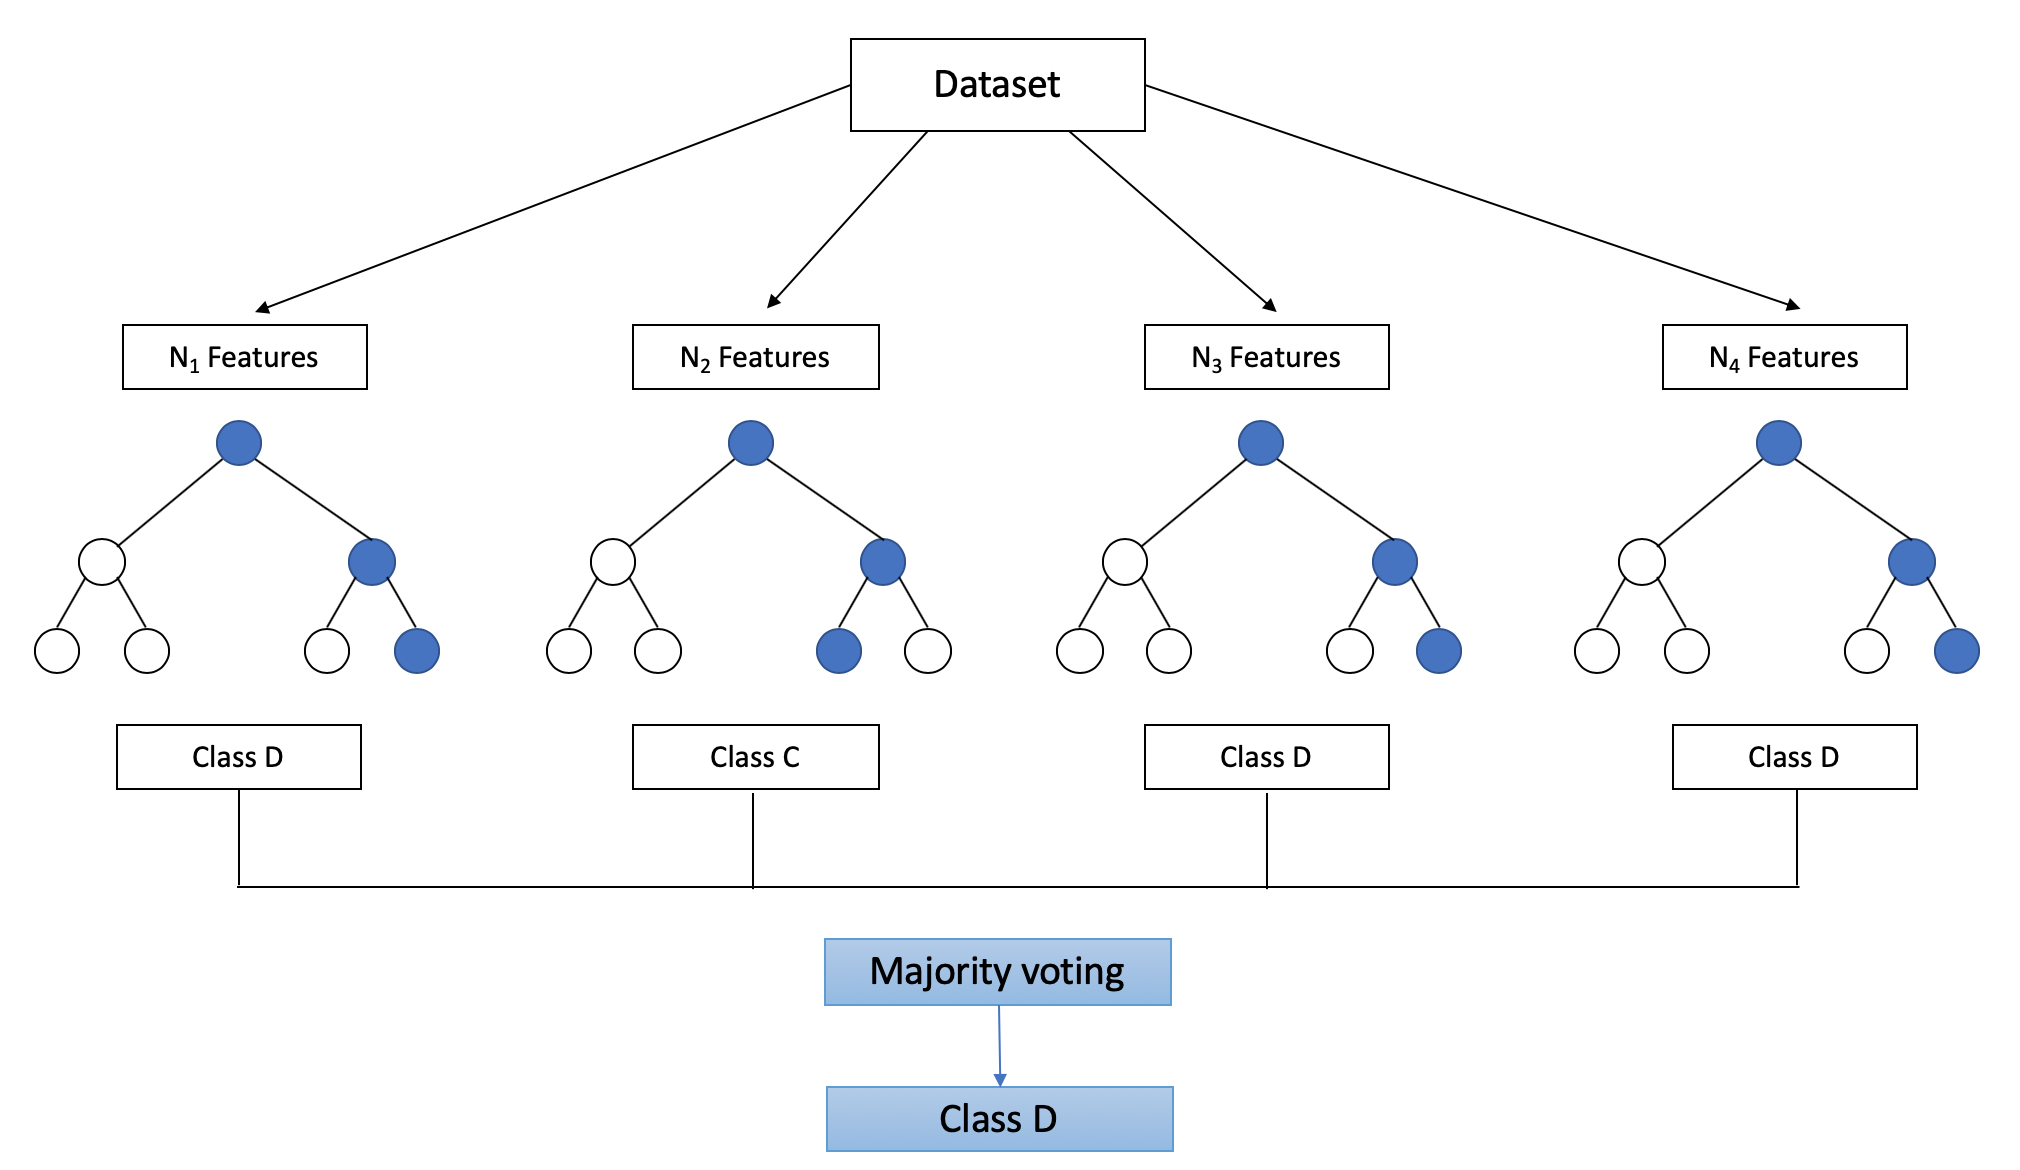
\includegraphics[width=0.8\textwidth]{images/random_forest.png}
	\caption{Darstellung \textit{Random Forest}}
	\label{fig:random_forest}
\end{figure}

\subsection{Hardware}
\label{sec:ml_hardware}

Die meisten Algorithmen für Künstliche Intelligenz, beziehungsweise speziell für \textit{Machine Learning}, sind sehr rechenaufwendig \cite{Du2018}. Grund dafür ist, dass sehr viele Daten verarbeitet werden müssen. Bei der Sub-Domäne \textit{Deep Learning} sind die Datenmengen noch mehr, da es sich hierbei meist um Bild-, Video- oder Audioaufnahmen handelt. Die darunterliegende Hardware ist daher von sehr großer Bedeutung, um Systeme effizient entwickeln, trainieren und einsetzten zu können.

Traditionelle Computersysteme wie \textit{Workstations} und Laptops sind anfangs die offensichtlichste Wahl für die Entwicklung. Es erlaubt eine schnelle Implementierung der ersten Ml-Modelle, welche kurzerhand gleich auf der lokalen \textit{Central Processing Unit} (CPU) validiert werden können. Dadurch ist auch eine hohe Flexibilität gegeben, was das Optimieren und Debuggen erleichtert. Dies funktioniert jedoch nur, wenn die Menge an Trainingsdaten überschaubar bleibt. Soll ein Modell für den Betrieb trainiert werden, kann es mitunter Tage oder sogar Wochen dauern, bis es fertig durchgerechnet ist. Die Architektur der CPU erlaubt es nämlich nicht, viele Berechnungen parallel auszuführen. Die \textit{Graphics Processing Unit} (GPU) hingegen bietet einen sehr hohen Parallelisierungsgrad, da Kalkulationen für Pixel und Matrizen meist einfach sind, aber oft durchzuführen sind. Bei \textit{Machine Learning} Algorithmen handelt es sich um ähnliche Aufgaben. Aufgrund dessen haben nach und nach immer mehr Entwickler GPUs für ML verwendet. Diesen Trend haben auch Hersteller erkannt und bieten GPUs mit spezieller Unterstützung für dieses Feld an.

Grafikkarten unterscheiden sich zu CPUs im Kontext von ML in drei großen Punkten. Erstens besitzen GPUs eine große Anzahl an kleinen Prozessoren, was die oben angesprochene Parallelisierung ermöglicht. Zweitens können viel höhere Datenmengen verarbeitet werden, da der lokale Speicher größer ist. Dadurch muss keine Zeit aufgewendet werden, um Daten von externen Speicherträgern zu laden, beziehungsweise zu schreiben. Das dritte Unterscheidungsmerkmal ist die Möglichkeit, \textit{floating point} Operationen durchführen zu können. Sie erlauben einen größeren Zahlenbereich bei der gleichen Anzahl an Bit. Vor allem hinsichtlich der Genauigkeit bringt dies einen Vorteil.

\textit{Field Progammable Gate Arrays} (FPGAs) ist eine andere Chipklasse, die immer populärer für ML wird \cite{Rebala2019}. Sowie GPUs stellen FPGAs eine hohe Rechenleistung und Parallelisierung bereit. Zu dem kommt noch ein viel höherer On-Chip Speicher mit einem generell geringeren Stromverbrauch. Weitere Vorteile sind, dass auch verschiedenartige Operationen gleichzeitig ausgeführt werden können und es eine Unterstützung von mehreren Datentypen gibt. Im Bereich funktionale Sicherheit sind diese Chips ausgereifter und werden daher häufiger für sicherheitskritische Applikationen wie Autonomes Fahren eingesetzt. Im Vergleich zu GPUs ist es komplexer, darauf aufbauende Software zu implementieren.

Das Unternehmen \textit{Google} hat für seine \textit{(Deep) Machine Learning} Anwendungen (Spracherkennung, Übersetzer, ...) einen eigenen \textit{Application-Specific Integrated Circuit} (ASIC) namens \textit{Tensor Processing Unit} (TPU) entworfen und entwickelt. Die Architektur unterscheidet sich in der von GPUs in dem Sinne, dass sie keine komplett parallelen Prozessoren besitzen, sondern lediglich ein Set von \textit{floating point} Instruktionen. Durch eine höchst effiziente Umsetzung sind TPUs 15 bis 30-mal schneller als GPUs bei einem geringeren Stromverbrauch. \textit{Tensor Processing Units} sind aber nicht käuflich zu erwerben und kommen daher nicht für einen lokalen Einsatzzweck infrage.

\subsection{Machine Learning-as-a-Service}
\label{sec:ml_as_a_service}

\textit{Machine Learning-as-a-service} (MLaaS) ist ein Überbegriff von \textit{Cloud}-basierten Technologien, welche für ML-Anwendungen benötigt werden. Es wird Datenvorbearbeitung, Trainieren und Validierung der Modelle, sowie der Betrieb zur Verfügung gestellt. Von \textit{Google} wird dies unter dem Namen \textit{Google Cloud AI} für Kunden angeboten \cite{Google2020}. Hierbei kommen die oben erwähnten TPUs mit dem hauseigenen AI Framework \textit{TensorFlow} zum Einsatz. Es werden drei Produkte unterschieden. \textit{AI Hub} ist ein Repository von Plug-and-Play Komponenten, die einen schnellen Einstieg ermöglichen und für eine bessere Zusammenarbeit innerhalb einer Organisation dienen. \textit{KI-Bausteine} sind unter anderem \textit{Vision AI} zur visuellen Erkennung, \textit{Natural Language} für z.B. Übersetzungen und \textit{AutoML Tables} für das strukturieren von Trainingsdaten. \textit{AI Platform} ist ein codebasierte Entwicklungsumgebung für ML-Entwickler.

Die \textit{Amazon Machine Learning} Dienste sind eine der automatisiertesten Lösungen in diesem Bereich \cite{Amazon2020}. Es werden binäre und multiclass Klassifikationen sowie Regression bereitgestellt. Der Kunde muss dabei lediglich die Zielvariable festlegen und im Hintergrund werden die Daten vorbearbeitet, der richtige Algorithmus ausgewählt und optimiert. Durch den hohen Automationsgrad geht jedoch die Flexibilität verloren. Deshalb gibt es auch \textit{SageMaker}, was eine eigene Umgebung für \textit{Data-Scientists} ist und zur Erstellung eigener Modelle dient.

\textit{Microsoft} hat mit \textit{Azure Machine Learning Studio} ebenfalls eine Lösung am Markt \cite{MS2020}. ML Studio ist dem Produkt von \textit{Amazon} sehr ähnlich. Jede Tätigkeit kann mittels \textit{drag and drop} durchgeführt werden. Dadurch ist eine geringe Lernkurve für Einsteiger gegeben. Mit über 100 Methoden für Klassifizierung und Regression, aber auch Anomalieerkennung wird dem Kunden sehr viel geboten.

Neben den genannten Unternehmen existieren noch \textit{IBM}, \textit{SAP}, \textit{BigML} sowie weitere. Jeder von ihnen stellt neben browserbasierten Oberflächen auch \textit{Representational State Transfer}-\textit{Application Programming Interfaces} (REST-APIs) zur Verfügung, mit denen Aufgaben automatisiert abgearbeitet werden können.

\section{CAN Bus}
\label{sec:can_bus}

Der \textit{Controller Area Network} Bus ist einer der bekanntesten Übertragungsmöglichkeiten in einem Fahrzeug und findet auch Verwendung in anderen Industrieanlagen wie beispielsweise Fahrstühlen \cite{Zimmermann2014}. Er verbindet mehrere Steuerungseinheiten (ECUs) zum Austausch von fahrzeugrelevanten Daten. Wie bereits in der Einführung erwähnt, sind typische Nachrichten die Motordrehzahl, Bremsdruck, Blinker etc. Es gibt jedoch auch eine Reihe von weiteren Bus-Systemen, welche im Einsatz sind, andere Anforderungen haben und für verschiedene Zwecke benötigt werden. Prominente Beispiele sind \textit{FlexRay}, \textit{LIN} und \textit{MOST}. Sie werden in sechs Klassen und nach Übertragungsrate eingeteilt (siehe Tabelle \ref{tab:bus_systems}).

\begin{table*}[htbp]
    \centering
    \caption{Klassifikation der Busssysteme nach Übertragungsrate \cite{Zimmermann2014}}
    \label{tab:bus_systems}
    \begin{tabular}{|l|l|l|l|}
        \hline
        Klasse & Bitrate & Typischer Vertreter & Anwendung \\
        \hline
        Diagnose & < 10 Kbit/s & ISO 9141 K-Line & Werkstatt- und Abgastester \\
        A & < 25 Kbit/s & LIN & \multirow{2}{*}{Karosserieelektronik}\\
        B & 25 ... 125 Kbit/s & CAN (Low Speed) & \\
        C & 125 ... 1000 Kbit/s & CAN (High Speed) & Antriebsstrang, Fahrwerk, ... \\
        D & > 1 Mbit/s & FlexRay & Bachbone-Netz \\
        Infotainment & > 10 Mbit/s & Ethernet & Multimedia \\
        \hline
  \end{tabular}
\end{table*}

Der CAN Bus wurde in den 1980er Jahren vom Unternehmen \textit{Bosch} mit dem Ziel entwickelt, die Kabelbäume zu verkürzen, um so Gewicht und Material zu sparen. Damals wurden bis zu 2 km Kabel in Fahrzeugen eingezogen, was mit der steigenden Anzahl an Steuergeräten mehr und mehr geworden wäre, da die Verbindungen ausschließlich Punkt zu Punkt waren. Seit 1991 findet der Bus als erstes den Einzug in Klasse C-Netze und stellt seither die Spezifikation für die Basis jeglicher CAN-Implementierungen dar. Die Konzipierung des Buses ist so ausgelegt, dass eine hohe Fehlersicherheit bei kurzen Botschaftslängen für einen Echtzeitbetrieb gegeben ist.

In der Tabelle ist ersichtlich, dass der Einsatzbereich auch in der Klasse B liegt, welche die Komfort-Systeme umfasst. Generell wird zwischen High- und Low-Speed unterschieden. Die Übertragungsrate des High-Speed-CAN ist bei 125 Kbit bis zu 1 Mbit pro Sekunde. Er verbindet maximal 20 ECUs des Antriebsstrangs (Motorelektronik, Getriebe- und Lenkradsteuerung, ABS, etc.). Aufgrund der hohen Sicherheitsrelevanz ist eine möglichst robuste Datenübertragung gefordert. Ein Fehler gerade im Automotive-Bereich könnte verheerende Folgen haben, wenn es dadurch zu einem Unfall kommt. Der Low-Speed-Can ist hingegen nicht so sicherheitskritisch, da vorwiegend Steuergeräte für zum Beispiel die Scheibenwischer, Zentralverriegelung oder Klimaanlage vernetzt werden. Die Datenrate beschränkt sich bei diesem Bus auf maximal 125 Kbit/s bei maximal 30 Knoten.

Die höchstmögliche Geschwindigkeit von einem Mbit pro Sekunde kann jedoch nur bei einer Strecke mit bis zu 40 Metern erreicht werden. Je länger die Kabel werden, desto geringer wird die Übertragungsrate. Der Grund für diese Einschränkung liegt bei der gleichzeitigen Datenverarbeitung von Busteilnehmern. Tabelle \ref{tab:can_speed} zeigt weitere Längen zu Übertragungsraten.

\begin{table*}[htbp]
	\centering
	\caption{CAN Übertragungsrate zur Kabellänge}
	\label{tab:can_speed}
	\begin{tabular}{|l|l l l l l l l|}
			\hline
			Übertragungsrate [kbit/s] & 10 & 20 & 50 & 125 & 250 & 500 & 1000 \\
			\hline
			Kabellänge [m] & 6700 & 3300 & 1300 & 530 & 270 & 130 & 40 \\
			\hline
\end{tabular}
\end{table*}

In der CAN-Spezifikation ist im Wesentlichen nur der \textit{Data-Link Layer} beschrieben, was zu unterschiedlichen Umsetzungen des \textit{Physical Layer} geführt hat. Im Allgemeinen ist CAN ein bitstrom-orientierter Linien-Bus mit einer Zwei-Draht Leitung (CAN-High und CAN-Low). An beiden Enden muss der Bus mit einem 120 Ohm Widerstand terminiert werden, um Reflexionen zu verhindern.  Über beide Leitungen werden zwei komplementäre Signale übertragen, sodass bei einer Unterbrechung noch immer die Daten zugestellt werden können. Für die Übertragung selbst unterscheiden sich die Bit im Signalpegel. Eine logische \textit{1} wird hochohmig (\textit{rezessiv}) erzeugt und ein niederohmiges Signal (\textit{dominiant}) definiert eine logische \textit{0}.

\subsection{Data-Link Layer}

Der CAN-Bus ist ein \textit{Broadcast}-Medium, bei dem die Nachrichten keine Ziel-und Quelladresse inkludieren und jedes Steuergerät jede Nachricht empfängt. Die Botschaft beinhaltet stattdessen eine eindeutige Kennung, den \textit{Message Identifier}, durch welchen die ECUs entscheiden, ob sie eine Nachricht weiter verarbeiten oder verwerfen. Ursprünglich war die Kennung mit 11 Bit spezifiziert, aber aus Erweiterungsgründen wurde sie später auf 29 Bit festgelegt. Zusätzlich kommen noch 1 beziehungsweise 3 Steuerbits hinzu. Ein Steuergerät kann auf den Bus zugreifen, wenn mindestens drei Bitzeiten nichts gesendet/empfangen wurde. Dabei wird das CSMA/CR Verfahren mit Arbitrierung auf Basis von Prioritäten eingesetzt. Der \textit{Message Identifier} dient neben der Kennung hierfür auch als Angabe der Priorität einer Nachricht. Je niedriger die Zahl, desto höher die Priorität. Kommt es also auf dem Bus zu einer Kollision, "gewinnt" die Botschaft mit der höheren Kennung.

\begin{figure}[htbp]
	\centering
		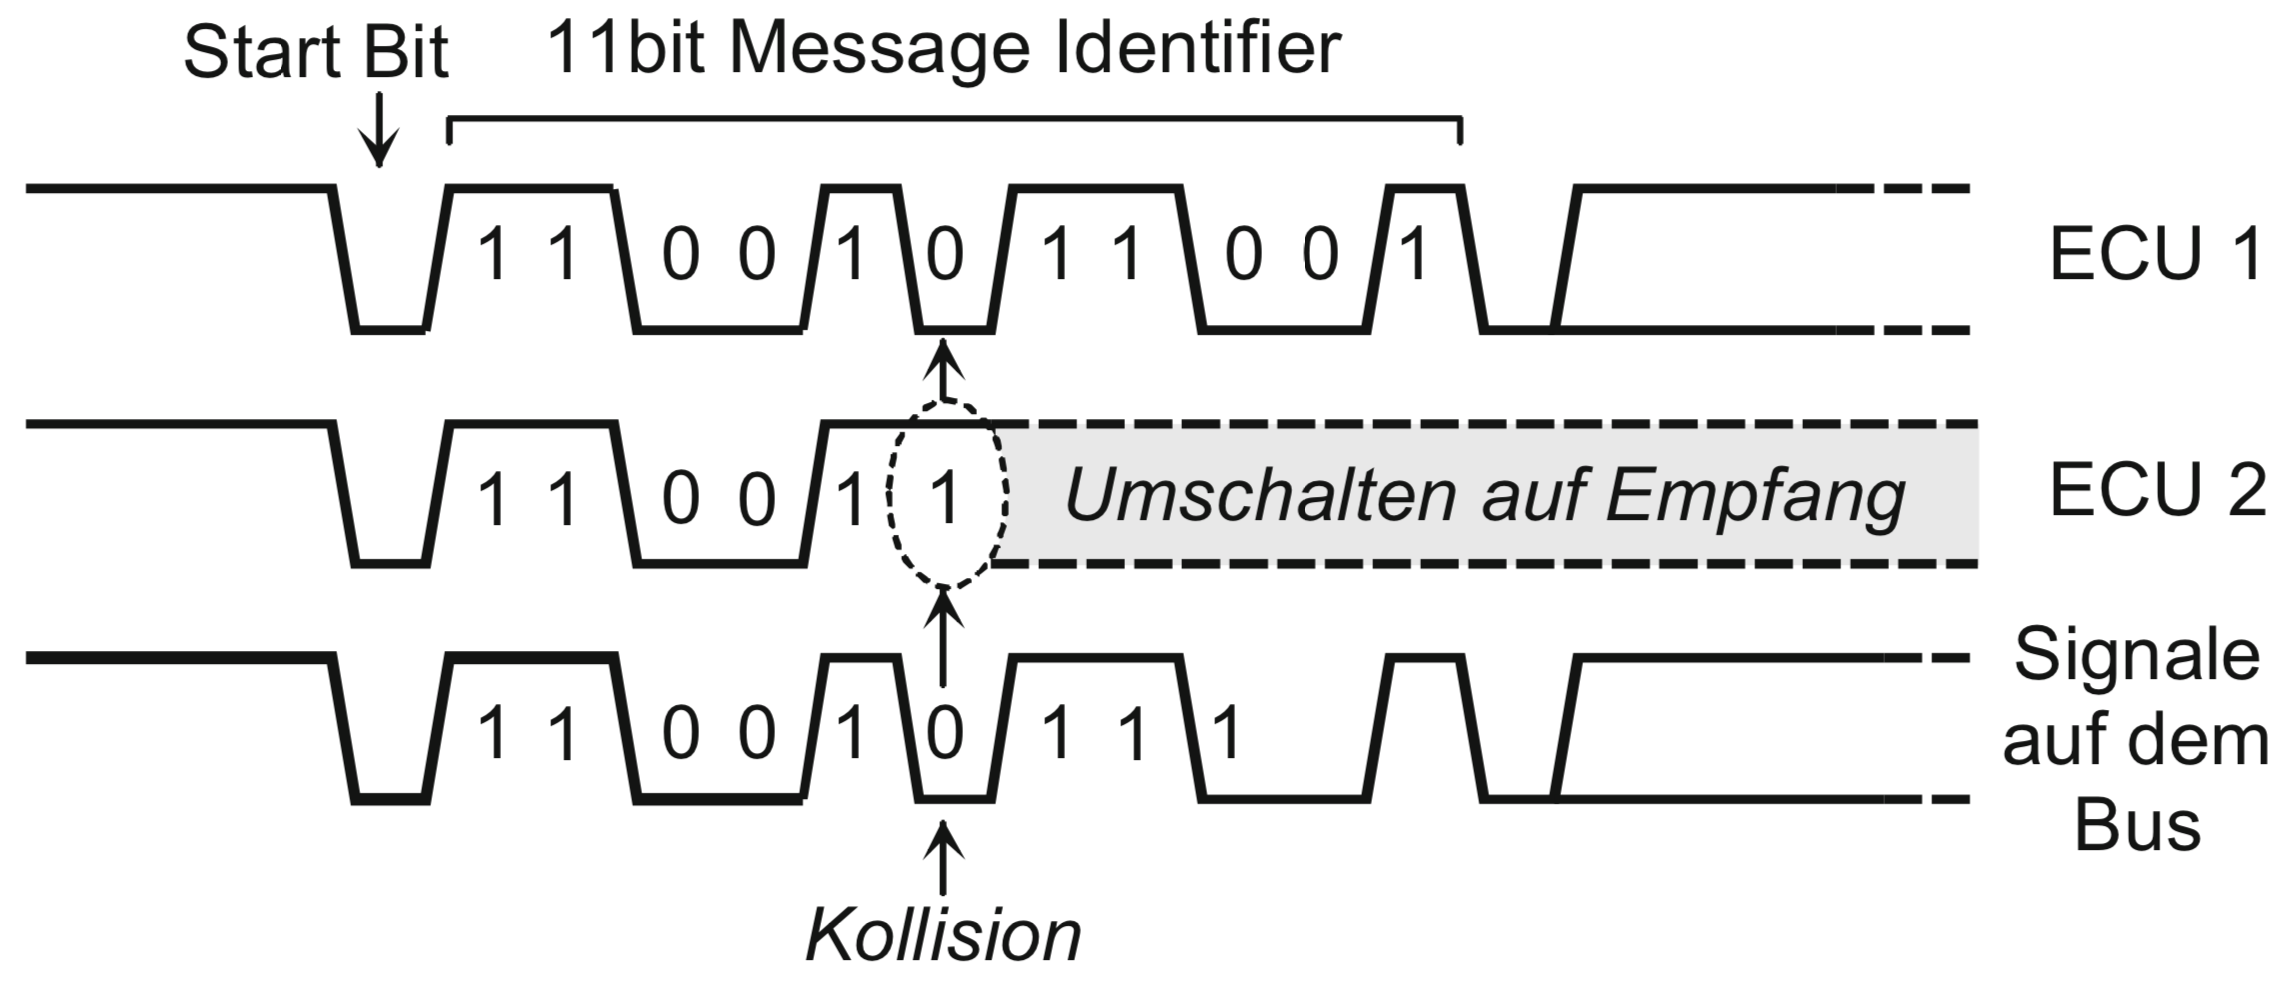
\includegraphics[width=0.6\textwidth]{images/can_csma_cr.png}
	\caption{Kollision von CAN-Nachrichten (Quelle: \cite{Zimmermann2014})}
	\label{fig:can_csma_cr}
\end{figure}

Abbildung \ref{fig:can_csma_cr} zeigt Verhalten, wenn zwei Steuergeräte gleichzeitig auf den Bus senden. ECU1 startet mit dem Senden des \textit{Message Identifiers} \textit{110 0101 1001}\textsubscript{B}, währendessen auch ECU2 mit der Kennung \textit{110 0111 0000}\textsubscript{B} beginnt. Beim sechsten Bit kommt es zu einer Kollision, da sich dort die Kennungen unterscheiden. Auf der Leitung dominiert jedoch die \textit{0}, da das Signal wesentlich niederohmiger im Vergleich zur \textit{1} ist. Die Steuergeräte überprüfen beim Senden, ob der Signalpegel auch dem jeweiligen gesendeten Bit entspricht und so erkennt ECU2, dass es zu einer Kollision gekommen ist. Es stellt sofort das Senden ein und auf Empfangen um. ECU1 führt das Übertragen unverzögert fort. Frühestens nach dem Ende der Nachricht und drei freien Bitzeiten versucht das zweite Steuergerät das erneute Versenden.

Die \textit{Payload} einer CAN-Nachricht kann zwischen null und acht Byte lang sein, wobei die Anzahl im \textit{Data Length Code} (DLC) Feld innerhalb der \textit{Control Bits} steht. Eine 15 Bit lange Prüfsumme (\textit{Cyclic Redundancy Check}, CRC) dient zur Fehlererkennung. Die Bitgeneratoren der Empfänger synchronisieren sich mithilfe des Startbits des Senders und werden durch zusätzlich eingefügte \textit{Stuff-Bits} nachsynchronisiert. Nachdem ein CAN-Controller eine Nachricht empfangen hat, wird das Paketformat und der CRC-Code überprüft. Stimmt alles überein, sendet der Controller innerhalb des \textit{Acknowledge und End of Frame} Felds eine positive Empfangsbestätigung. Andernfalls ein \textit{Error Frame}, was zu einem Ignorieren der Nachricht bei allen anderen Empfängern führt. Dadurch ist gewährleistet, dass die Daten am Bus und der Teilnehmer konsistent bleiben. Der Sender, bei dem es zu einem Fehler gekommen ist, startet automatisch einen neuen Versuch. Abbildung \ref{fig:can_packet} fasst das CAN-Nachrichtenformat noch einmal zusammen.

\begin{figure}[htbp]
	\centering
		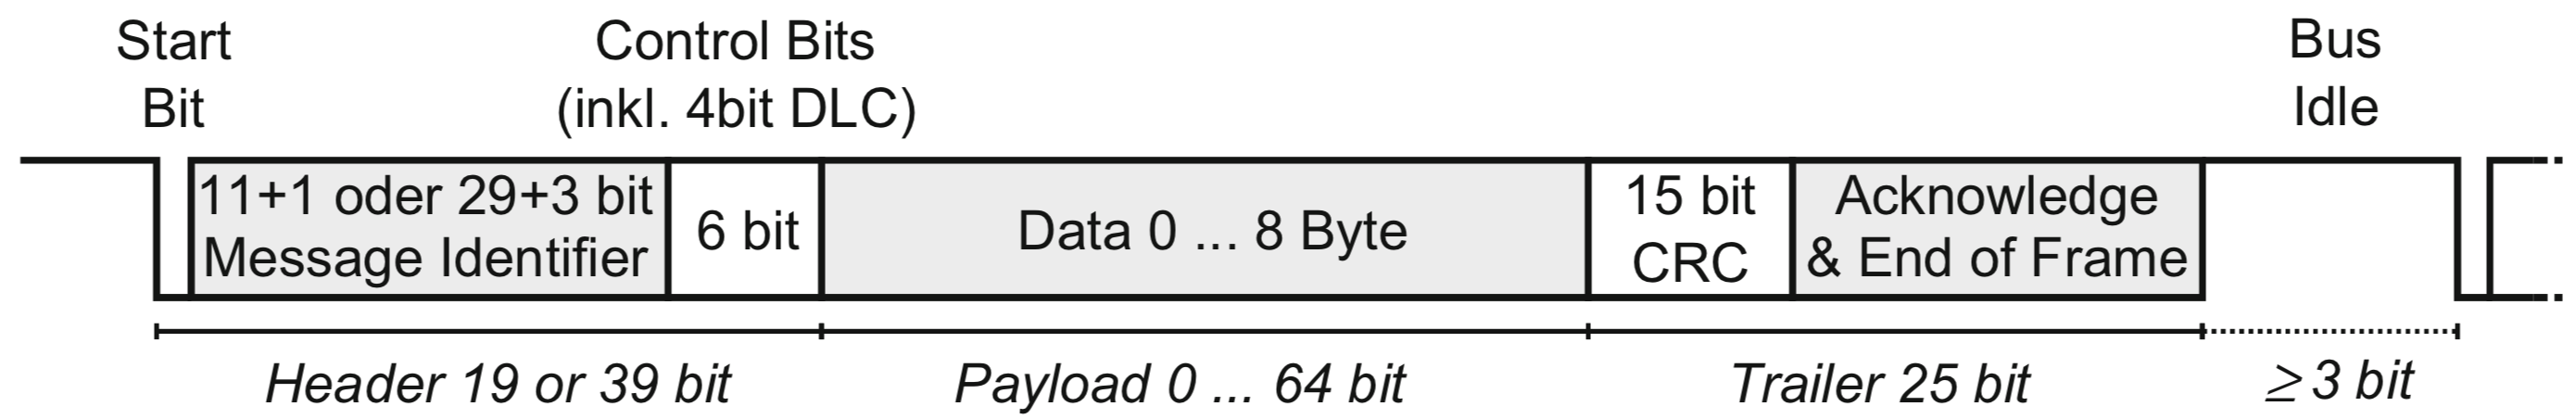
\includegraphics[width=0.8\textwidth]{images/can_packet_format.png}
	\caption{CAN-Paketformat (Quelle: \cite{Zimmermann2014})}
	\label{fig:can_packet}
\end{figure}

\subsection{Fehlerbehandlung}

Durch diese Fehlererkennungsverfahren ergibt sich eine hohe Übertragungszuverlässigkeit. Viele verschiedene Untersuchungen haben eine Restfehlerwahrscheinlichkeit von 10\textsuperscript{-11} ausgemacht. Auch die Übertragungswiederholung tritt sehr schnell ein, da spätestens am Ende einer Botschaft die Erkennung eines möglichen Fehlers vorliegt. Zusätzlich hat jeder CAN-Controller einen eigenen Fehlerspeicher, in dem Sende- und Empfangsfehler protokolliert werden. Dabei wird unterschieden, ob nur der Controller selbst einen Fehler erkennt, oder ob ihn auch andere feststellen. Erkennt ein Steuergerät, dass wiederholt Sendefehler erzeugt werden, stellt es als ersten Schritt das Senden ein. Kann das Problem mithilfe einer Fehler-Ursachen-Analyse und -Behebung nicht gelöst werden, schaltet sich das Gerät vollständig ab. Dies wird unter dem Begriff \textit{Bus off} verstanden. Tritt jedoch vielleicht nur eine vorübergehende Störung durch elektromagnetische Effekte (EMV-Störung) auf, geht das Steuergerät wieder in Normal-Betrieb über, nachdem diese vorbei sind. Die Anzahl der Fehler, welche toleriert werden und Zeit die verstreichen darf ist entweder von Standards beziehungsweise von der Gesetzgebung vorgeschrieben oder durch den Hersteller festgelegt.

\subsection{CAN Matrix}

Die CAN-Spezifikation gibt keinerlei Vorgaben für Nachrichtenkennungen, Formatierung oder Bedeutung der zu sendenden Nachrichten. Dadurch ist eine sehr hohe Flexibilität und geringer Overhead gegeben, welcher auch für eine solche Umgebung notwendig ist. So legt jeder \textit{Original Equipment Manufacturer} (OEM) oder Zulieferer die Punkte für sich individuell selbst fest. Sie müssen nur innerhalb eines Fahrzeuges einheitlich auf allen Steuergeräten umgesetzt sein. Dies beinhaltet folgendes:

\begin{itemize}
	\item welche Steuergeräte welche CAN-Nachrichten unten welchen Bedingungen senden/verarbeiten
	\item den \textit{Message Identifier} bzw. die Priorität der Nachrichten
	\item mit welchem Zyklus gesendet wird
	\item welche Daten oder Signale enthalten sind
	\item die Normierung der Daten, bzw. die Umrechnungsbeziehung zwischen den Rohdaten und den physikalischen/logischen Größen
\end{itemize}

All diese Informationen sind in der sogenannten CAN-Matrix (CAN-Datenbank, CANdb, DBC-Datei) enthalten und sind auf jedem Busteilnehmer zu implementieren. Erst mit einer solchen Datei ist es möglich, den CAN-Datenstrom auszuwerten und im Netzwerk teilzunehmen. Das Listing \ref{lst:dbc_snippet} zeigt einen Ausschnitt eines DBC-Files mit dem Signal \textit{Bremsdruck}.

\begin{lstlisting}[frame=lines, caption=Ausschnitt CAN DBC-File, captionpos=b, label = lst:dbc_snippet, showstringspaces=false, basicstyle=\footnotesize]
BO_ 262 ESP_05: 8 Bremse_ABS_MK100
    ...
    SG_ ESP_Schwelle_Unterdruck : 14|2@1+ (1.0,0.0) [0.0|3] ""  Gateway_MQB
    SG_ ESP_Bremsdruck : 16|10@1+ (0.3,-30) [-30.0|276.6] "Unit_Bar"  Allrad_Haldex_TT3,Daempfer,Gateway_MQB,Lenkhilfe_EPS,Magnetic_Ride,PDC_PLA,PDC_PLA_ARA
    SG_ ESP_Fahrer_bremst : 26|1@1+ (1.0,0.0) [0.0|1] ""  Allrad_Haldex,Allrad_Haldex_TT3,Gateway_MQB,Lenkhilfe_EPS,VAQ
    ...
\end{lstlisting}

In der ersten Zeile ist die CAN-Nachricht definiert. \textit{262} ist der \textit{Message Identifier}, \textit{ESP\_05} heißt die Nachricht, die Länge (DLC) ist \textit{8} und wird von dem Steuergerät \textit{Bremse ABS MK100} versendet. Die Zeilen darunter spezifizieren die Signale, welche in der Nachricht enthalten sind. Anfangs steht die Bezeichnung, nach dem ":" die Stelle des ersten Bits und die Anzahl der Bit. Die restlichen Felder legen die Skalierung, das Offset, das Minimum und das Maximum, sowie, falls vorhanden, die Einheit fest. Am Ende werden alle Steuergeräte gelistet, welche das Signal weiterverarbeiten dürfen.

\subsection{MDF}

\textit{Measurement Data Format} (MDF) \cite{ASAM14} ist ein binäres Dateiformat, welches 1991 von der Firma \textit{Vector Informatik GmbH} in Zusammenarbeit mit der \textit{Robert Bosch GmbH} entwickelt wurde. Es ist speziell für Messdaten im Automotive-Bereich konzipiert und ist seit 2009 in der Version 4 als offizieller Standard von \textit{Association for Standardization of Automation and Measuring Systems} (ASAM) öffentlich zugänglich. Ein wesentlicher Vorteil des Formates ist, dass die Messdaten sehr schnell und speicherplatzsparend abgespeichert werden können. Des Weiteren wird auch eine Optimierung des Lesevorgangs durch Vorsortierung und Indizierung unterstützt. Neben den eigentlichen Nutzdaten werden auch Metadaten aus der DBC-Datei mitgespeichert. Dies ist vor allem für weitere Analysen und die Interpretation der Rohdaten notwendig. Beispielsweise gehören dazu die Information zur Umwandlung in physikalische Werte und Signalnamen.

\section{Edge Computing}
\label{sec:edge_computing}

\textit{Cloud Computing} hat einen enormen Einfluss auf das tägliche Leben und die Arbeitswelt in den verschiedensten Bereichen genommen. \textit{Software-as-a-Service} (SaaS) Produkte wie die \textit{Google-Apps}, \textit{Social Media}, \textit{Github}, \textit{Office 365} sowie das Verarbeiten von großen Datenmengen für \textit{Machine Learning} Anwendungen sind kaum mehr wegzudenken, beziehungsweise zu realisieren ohne dieser Möglichkeit. Zudem sind viele Unternehmen auf die Infrastrukturen der \textit{Cloud} (\textit{Infrastructure-as-a-Service}, IaaS) angewiesen, um den Betrieb aufrecht erhalten zu können \cite{Shi2016}. Mit dem Aufmarsch der IoT ist die \textit{Post-Cloud}-Ära angebrochen, in der mit dem Internet verbundene Geräte Daten erzeugen, verteilen aber auch speichern, analysieren und verwenden. Mit dem Jahr 2020 prognostiziert Cisco 50 Milliarden IoT-Geräte, deren Anwendungen kurze Antwortzeiten brauchen, persönliche Daten verarbeiten oder so eine große Datenmenge erzeugen, dass es eine Herausforderung für die Netzwerke darstellt \cite{Evans2011HowTN}. Da es dann meist der Fall ist, dass dieselben Geräte wiederum Daten von der \textit{Cloud} empfangen und darauf zum Beispiel eine Aktion setzen, macht es Sinn, die Daten gleich an der selben Stelle zu verarbeiten. Dies wird unter \textit{Edge Computing}, also dem Erzeugen, Auswerten und Verarbeiten von Daten an dem äußersten Knoten des Netzwerks, verstanden \cite{Shi2016}.

Den ganzen Rechenaufwand in die \textit{Cloud} auslagern hat sich für die letzten Jahre als eine effiziente und praktikable Lösung erwiesen. Je mehr Daten jedoch von IoT-Geräten erzeugt und an Rechenzentren gesendet werden, desto eher kommt es zu einem Flaschenhals bei den Transportwegen. Das resultiert unmittelbar in einer höheren Latenz und wirkt sich in weiterer Folge auf eine schlechte Benutzererfahrung der Anwendungen aus. Selbstfahrende Autos zeigen ein zusätzliches Problem, das daraus entsteht, auf. Sie generieren pro Sekunde ein Gigabyte an Messdaten, auf Basis dessen in Echt-Zeit eine Entscheidung getroffen werden soll \cite{CW13}. Bei einer Übertragung all dieser Daten würde die Antwort zu lange auf sich warten lassen. Einerseits stößt das lokale Funknetz in Sachen Bandbreite, Zuverlässigkeit und Verfügbarkeit an seine Grenzen, wenn viele Autos es gleichzeitig tun. Andererseits können selbst im größten Rechenzentrum nicht alle Anfragen zeitgleich und schnellstmöglich abgearbeitet werden, sodass eine weitere Wartezeit hinzukommt. Die Autos wären somit kaum imstande eine Entscheidung rechtzeitig umzusetzen, welche womöglich einen Unfall verhindert. Eine Gruppe von Forschern \cite{Yi15} hat einen \textit{Proofe-of-Concept} (PoC) mit Bildanalysen vorgestellt, bei dem die Antwortzeit von 900 auf 169 Millisekunden verkürzt werden konnte, indem die Auswertungen von der \textit{Cloud} zum Rande des Netzwerkes verlagert wurden.

Der nächste Punkt, der in \textit{Edge Computing} eine Rolle spielt, ist der Datenschutz (engl. \textit{Privacy}). In einem \textit{Smart Home} kann beispielsweise über den Wasser- und Energieverbrauch festgestellt werden, wie viele Personen sich in dem Haushalt momentan aufhalten. Normalerweise erfolgt die Datenspeicherung und eventuell die Auswertung in der \textit{Cloud}, was natürlich mehr Angriffsvektoren bietet. Hierbei verbleiben aber alle Daten sozusagen im Haus und werden nur lokal verarbeitet, jedoch müssen selbstverständlich auch hier Vorkehrungen bezüglich Datensicherheit getroffen werden. \textit{Wearables} haben zudem noch Zugriff auf Gesundheitsdaten, welche sehr sensible personenbezogene Daten sind. Die Geräte schicken diese zum \textit{Service Provider} für die Speicherung und Aufbereitung. Geschieht der Schritt nicht und die Daten bleiben am Gerät, wo die Benutzerin stets volle Kontrolle darüber hat, ist es leichter, Datenschutz gewährleisten zu können. Der Anwender kann sich weiterhin dazu entschließen, die Daten in die \textit{Cloud} zu senden, um etwaige Dienste zu konsumieren. Essentiell bleibt aber, dass eben die Eigentümerin darüber entscheidet, was mit ihren Daten passiert.

IoT-Geräte beziehungsweise Geräte, welche sich am Rande des Netzwerks befinden, sind oft nicht an das lokale Stromnetz angebunden und so stellt die Batterie eine ausschlaggebende Ressource dar. Alle Berechnungen in die \textit{Cloud} auszulagern hilft dabei Energie zu sparen. Das Übertragen der Daten benötigt jedoch vor allem mit WLAN auch einen hohen Energieaufwand. Hier fließt folgendes mit ein: Um wie viele Daten handelt es sich? Wie oft werden die Daten gesendet? Wie gut ist die Signalstärke? Welche Bandbreite steht zur Verfügung? Soll der Energieverbrauch des gesamten Kommunikationsweges einfließen? Erst wenn all diese Fragen beantwortet sind, kann der Energieverbrauch zur lokalen Verarbeitung gezogen werden. Laut der Literatur \cite{Shi2016} ist es bei vielen Anwendungen günstiger, zweiteres umzusetzen.